\documentclass[journal]{IEEEtran}

\usepackage{cite}
\usepackage{amsmath,amssymb,amsfonts,amsthm,bm,mathtools}
\usepackage{graphicx}
\usepackage{booktabs,multirow,array}
\usepackage{algorithm}
\usepackage{algpseudocode}
\usepackage{url}
\usepackage{color}
\usepackage{balance}

\graphicspath{{../figs/}}

\newtheorem{proposition}{Proposition}
\newtheorem{remark}{Remark}

\begin{document}

\title{EE-SE Pareto Frontier and Amplification Structure Optimization for Hybrid Active-Passive STAR-RIS}

\author{Anonymous Authors}

\maketitle

\begin{abstract}
Hybrid active-passive simultaneously transmitting and reflecting reconfigurable intelligent surfaces (STAR-RISs) can enlarge the spectral-efficiency (SE) region of fully passive STAR-RISs, yet their energy-efficiency (EE) gains remain poorly understood because three ingredients are usually oversimplified: amplifier-noise injection, control/switching power, and the asymmetric transmission/reflection tasks intrinsic to STAR operation. This paper develops a structured and analytically transparent framework for the EE-SE frontier of hybrid active-passive STAR-RIS. First, we introduce a three-part power model that separates static controller/bias consumption, dynamic state-switching overhead, and communication-side transmit/amplification power. Second, for a sparse active set and side-wise common gains, we derive a closed-form SE-optimal amplification structure and an explicit active-on threshold showing when amplification is beneficial. Third, we characterize the Pareto boundary through an $\epsilon$-constraint formulation with an outer sparse-activation search and an inner closed-form gain/rate-split update. The resulting design rules are protocol-aware and directly reveal how amplifier noise, side-wise power splitting, and hardware overhead reshape the frontier. Numerical results averaged over $30$ channel draws show that, at $12$ bit/s/Hz, the proposed sparse-hybrid design improves EE by about 24.1\%, 62.8\%, and 59.3\% over uniform hybrid, fully active, and passive baselines, respectively, while remaining feasible up to $20$ bit/s/Hz under the considered budget. The main outcome is a transferable answer to when active elements should be turned on, how many should be activated, and how much gain they should use.
\end{abstract}

\begin{IEEEkeywords}
STAR-RIS, active RIS, hybrid active-passive RIS, energy efficiency, spectral efficiency, Pareto frontier, amplifier noise.
\end{IEEEkeywords}

\section{Introduction}
Reconfigurable intelligent surfaces (RISs) are a central enabler of 6G smart radio environments because they reshape propagation with very low hardware complexity compared with conventional relays and active repeaters \cite{direnzo2020smart,huang2019ee,wu2019irs,tang2020mimo}. Simultaneously transmitting and reflecting RISs (STAR-RISs) further extend passive beam manipulation from one-sided reflection to $360^\circ$ coverage, enabling distinct user groups on the transmission and reflection sides to be served by a common surface \cite{liu2021star,mu2022star,zuo2021noma}. This dual-side coverage benefit is especially attractive when transmission-side and reflection-side users have different path losses, quality-of-service (QoS) targets, and scheduling roles.

A persistent limitation, however, is the multiplicative path loss of purely passive surfaces. Active and hybrid active-passive RIS architectures alleviate this loss by embedding a small number of amplifying elements, but they also inject amplifier noise and incur non-negligible bias power \cite{ma2023activeee,gao2023active,kunzan2022sub,qi2022sub,peng2023hybrid,huang2024hybrid,nguyen2024uav,zhang2022signal}. Recent measurement-driven studies further show that RIS power consumption is not a single constant; it contains static controller power, technology-dependent per-element consumption, and dynamic state-switching overhead \cite{wang2023static,wang2024practical,fotock2024active}. These observations become even more consequential for STAR-RIS because transmission and reflection generally serve different tasks and thus compete for the surface aperture, side-wise power split, and active hardware budget.

Despite rapid progress, three gaps remain open. \emph{First}, the noise injected by active elements is often modeled coarsely, so there is still no transferable rule explaining when active mode should be used, how many active elements are needed, and whether they should preferentially support the transmission or reflection side. \emph{Second}, EE conclusions are frequently based on oversimplified power models, which makes them difficult to map to the control and hardware layers. \emph{Third}, existing hybrid active-passive STAR-RIS studies are still dominated by numerical optimization, while structural frontier characterizations and protocol-aware insights for energy splitting (ES), time switching (TS), and space splitting (SS) are scarce \cite{vu2025hybridstar,song2025prototype,zhu2025activepassive,soleymani2023starurlcc,xue2023maxmin,zhang2024activestarisac}.

To this end, we develop a structured post-ZF equivalent formulation that preserves the hybrid STAR-RIS model while yielding tractable frontier characterizations. The main contributions are as follows.
\begin{itemize}
    \item We formulate a hybrid active-passive STAR-RIS downlink with transmission-side users and reflection-side users, and we introduce a three-part power model including static controller/bias power, dynamic switching power, and communication-side BS/amplifier power.
    \item For a fixed active set, we derive an equivalent side-wise SINR model. The resulting SE-optimal common amplification factor admits a closed-form expression, and the derivative yields an explicit \emph{active-on threshold} that quantifies when the coherent-gain benefit dominates amplifier-noise injection.
    \item We develop a structured sparse-activation solver whose outer selection, side-aware weighting, closed-form gain update, and target-rate inversion remain analytically consistent with the proposed framework. This yields a low-complexity alternative to mixed-integer nonlinear programming.
    \item We reveal concrete design rules: passive STAR-RIS is competitive at low SE, sparse hybrid activation is preferable at moderate-to-high SE, the optimal active ratio grows from about 0.14 at $8$ bit/s/Hz to about 0.68 at $20$ bit/s/Hz, and stronger amplifier noise reduces the preferred gains and narrows the EE region.
\end{itemize}

\section{System Model}
\subsection{Hybrid active-passive STAR-RIS downlink}
Consider a BS with $M$ antennas serving $K_t$ users on the transmission side and $K_r$ users on the reflection side via an $N$-element STAR-RIS. Let $\mathcal{K}_t=\{1,\ldots,K_t\}$ and $\mathcal{K}_r=\{1,\ldots,K_r\}$. Under the ES protocol, the $n$th STAR-RIS element uses transmission/reflection coefficients
\begin{equation}
\theta_{n,s}=\sqrt{\rho_{n,s}}\eta_{n,s}e^{j\phi_{n,s}},\qquad s\in\{t,r\},
\label{eq:theta}
\end{equation}
with $\rho_{n,t}+\rho_{n,r}=1$, $0\le \rho_{n,s}\le 1$, and $1\le \eta_{n,s}\le \beta_{\max}$. For passive elements, $\eta_{n,s}=1$; for active elements, $\eta_{n,s}=\beta_{n,s}>1$ on the assigned side. Let $\mathcal{A}_t$ and $\mathcal{A}_r$ denote the active-element sets for transmission and reflection, and let $\mathcal{A}=\mathcal{A}_t\cup\mathcal{A}_r$.

Denote by $\mathbf{G}\in\mathbb{C}^{N\times M}$ the BS-to-STAR-RIS channel, and by $\mathbf{h}_{s,k}\in\mathbb{C}^N$ the STAR-RIS-to-user channel on side $s$ for user $k$. The received signal of user $(s,k)$ is
\begin{equation}
y_{s,k}=\mathbf{h}_{s,k}^H\mathbf{\Theta}_s\mathbf{G}
\sum_{j\in\mathcal{K}_s}\mathbf{w}_{s,j}x_{s,j}
+\mathbf{h}_{s,k}^H\mathbf{n}_{a,s}+n_{s,k},
\label{eq:received}
\end{equation}
where $\mathbf{\Theta}_s=\mathrm{diag}(\theta_{1,s},\ldots,\theta_{N,s})$, $\mathbf{w}_{s,j}$ is the BS beamformer for user $(s,j)$, $x_{s,j}$ is the unit-power information symbol, $n_{s,k}\sim\mathcal{CN}(0,\sigma_0^2)$ is thermal noise, and $\mathbf{n}_{a,s}$ collects the amplifier noises of the active elements on side $s$. The SINR of user $(s,k)$ becomes
\begin{equation}
\gamma_{s,k}=
\frac{\left|\mathbf{h}_{s,k}^H\mathbf{\Theta}_s\mathbf{G}\mathbf{w}_{s,k}\right|^2}
{\sum_{j\neq k}\left|\mathbf{h}_{s,k}^H\mathbf{\Theta}_s\mathbf{G}\mathbf{w}_{s,j}\right|^2
+\sigma_{a,s,k}^2+\sigma_0^2},
\label{eq:sinr_full}
\end{equation}
where $\sigma_{a,s,k}^2$ is the active-noise term seen at user $(s,k)$ and is proportional to the active gains and the corresponding STAR-RIS-user channel strengths.

\subsection{Three-part power-consumption model}
Motivated by recent measurement-based RIS power studies \cite{wang2023static,wang2024practical}, we write the total consumed power as
\begin{equation}
\begin{aligned}
P_{\mathrm{tot}}
&=\frac{1}{\eta_{\mathrm{PA}}}
\sum_{s\in\{t,r\}}\sum_{k\in\mathcal{K}_s}\|\mathbf{w}_{s,k}\|^2
+P_{\mathrm{ctrl}}+P_{\mathrm{bias}}|\mathcal{A}|  \\
&\quad +f_u\!\left(P_{\mathrm{sw},0}+P_{\mathrm{sw},1}|\mathcal{A}|\right) \\
&\quad +\sum_{n\in\mathcal{A}_t}\mu_t(\beta_{n,t}^2-1)
+\sum_{n\in\mathcal{A}_r}\mu_r(\beta_{n,r}^2-1),
\end{aligned}
\label{eq:power_model}
\end{equation}
where the first term is the BS radiated power divided by PA efficiency $\eta_{\mathrm{PA}}$, $P_{\mathrm{ctrl}}$ is the controller power, $P_{\mathrm{bias}}$ captures static per-active-element biasing, $f_u$ is the state-update frequency, and the last two sums describe the amplification-dependent power. This decomposition explicitly distinguishes static, dynamic, and communication-side costs; as shown later, these three parts dominate different operating regions of the EE-SE tradeoff.

\subsection{Structured post-ZF equivalent formulation}
To obtain interpretable structure, we adopt a post-ZF equivalent model. Specifically, the BS uses side-wise zero-forcing directions and only the scalar user powers remain to be allocated. The STAR-RIS phases are aligned to the dominant cascaded paths, and all active elements on the same side share a common gain $\beta_s$. Let $g_n$ be the effective BS-to-element channel after post-ZF projection, and let $h_{s,k,n}$ be the $n$th entry of $\mathbf{h}_{s,k}$. Define the coherent gain proxy
\begin{equation}
u_{s,k,n} = |g_n|\,|h_{s,k,n}|.
\label{eq:un}
\end{equation}
Then the side-wise effective coherent term for user $(s,k)$ is
\begin{equation}
\psi_{s,k}(\beta_s)=
\sum_{n\in\mathcal{P}_s}\sqrt{\rho_s}u_{s,k,n}
+\beta_s\sum_{n\in\mathcal{A}_s}\sqrt{\rho_s}u_{s,k,n},
\label{eq:psi}
\end{equation}
where $\mathcal{P}_s=\{1,\ldots,N\}\setminus\mathcal{A}_s$ includes passive elements and the elements that are active for the opposite side but only passive for side $s$. The corresponding active-noise term is
\begin{equation}
\zeta_{s,k}(\beta_s)=\sigma_0^2+
\rho_s\beta_s^2\sigma_a^2
\sum_{n\in\mathcal{A}_s}|h_{s,k,n}|^2.
\label{eq:noise_exact}
\end{equation}
The minimum sum transmit power needed to satisfy a side target rate $R_s$ under equal user-rate splitting is then
\begin{equation}
p_s^{\min}(\beta_s)=
\sum_{k\in\mathcal{K}_s}
\frac{(2^{R_s/K_s}-1)\zeta_{s,k}(\beta_s)}{\psi_{s,k}^2(\beta_s)}.
\label{eq:minsidepower}
\end{equation}
The numerical implementation uses \eqref{eq:minsidepower} for power inversion together with the structural gain rule derived next.

\section{Problem Formulation}
The sum spectral efficiency is
\begin{equation}
R_\Sigma = \sum_{s\in\{t,r\}}\sum_{k\in\mathcal{K}_s}\log_2(1+\gamma_{s,k}),
\label{eq:sumrate}
\end{equation}
and the system energy efficiency is
\begin{equation}
\mathrm{EE} = \frac{R_\Sigma}{P_{\mathrm{tot}}}\quad \text{(bit/J)}.
\label{eq:ee}
\end{equation}
For completeness, the spectral-energy efficiency (SEE) is $\mathrm{SEE}=\mathrm{EE}/B$ when the bandwidth $B$ is explicitly retained.

The original EE-maximization problem can be written as
\begin{equation}
\begin{aligned}
\max_{\mathbf{W},\,\bm{\rho},\,\bm{\phi},\,\bm{\beta},\,\mathcal{A}}
\quad & \frac{R_\Sigma}{P_{\mathrm{tot}}} \\
\text{s.t.}\quad &
R_{s,k}\ge \bar{R}_{s,k},\ \forall s,k, \\
&
\sum_{s,k}\|\mathbf{w}_{s,k}\|^2 \le P_{\max}^{\mathrm{BS}},\\
&
1\le \beta_{n,s}\le \beta_{\max},\ \forall n\in\mathcal{A}_s,\\
&
\beta_{n,s}=1,\ \forall n\notin\mathcal{A}_s,\\
&
\rho_{n,t}+\rho_{n,r}=1,\ 0\le \rho_{n,s}\le 1,\\
&
\rho_{n,s}\beta_{n,s}^2\sigma_a^2 \le \Gamma_{n,s},\ \forall n,s,
\end{aligned}
\label{eq:P0}
\end{equation}
where $\Gamma_{n,s}$ is a maximum noise-injection or hardware-safety limit. Problem \eqref{eq:P0} is highly non-convex because of the fractional objective, binary active-set selection, and the multiplicative coupling between beamforming, STAR coefficients, and active noise.

To trace the EE-SE Pareto boundary, we adopt the $\epsilon$-constraint formulation
\begin{equation}
\begin{aligned}
\mathcal{P}(\epsilon):\quad
\min_{\mathbf{W},\,\bm{\rho},\,\bm{\phi},\,\bm{\beta},\,\mathcal{A}}
\quad & P_{\mathrm{tot}} \\
\text{s.t.}\quad &
R_\Sigma \ge \epsilon, \\
& \text{constraints of \eqref{eq:P0}.}
\end{aligned}
\label{eq:epsilon}
\end{equation}
Every feasible solution of \eqref{eq:epsilon} yields one point on the Pareto frontier. The remaining question is how to solve \eqref{eq:epsilon} with enough structure to produce transferable design rules.

\section{Optimal Structure of the Amplification Factors}
\subsection{Equivalent side-wise SINR law}
For a fixed active set and fixed phase alignment, define
\begin{equation}
a_s=\min_k \sum_{n\in\mathcal{P}_s}\sqrt{\rho_s}u_{s,k,n},\qquad
b_s=\min_k \sum_{n\in\mathcal{A}_s}\sqrt{\rho_s}u_{s,k,n},
\label{eq:ab}
\end{equation}
and
\begin{equation}
c_s=\sigma_0^2,\qquad
d_s=\max_k \rho_s\sigma_a^2\sum_{n\in\mathcal{A}_s}|h_{s,k,n}|^2.
\label{eq:cd}
\end{equation}
With average side power $\bar{p}_s$, a conservative worst-user SINR lower bound is
\begin{equation}
\underline{\gamma}_s(\beta_s)=
\frac{\bar{p}_s(a_s+b_s\beta_s)^2}{c_s+d_s\beta_s^2}.
\label{eq:surrogate}
\end{equation}
Equation \eqref{eq:surrogate} isolates the key conflict: coherent signal growth is linear in $\beta_s$, while injected active noise grows quadratically.

\begin{proposition}
For fixed $(a_s,b_s,c_s,d_s)$ with $a_s>0$, $c_s>0$, and $d_s>0$, the function $\underline{\gamma}_s(\beta_s)$ in \eqref{eq:surrogate} is unimodal over $[1,\beta_{\max}]$, and its SE-optimal gain is
\begin{equation}
\beta_{s,\mathrm{SE}}^\star=
\left[\frac{b_sc_s}{a_sd_s}\right]_{[1,\beta_{\max}]},
\label{eq:beta_closed}
\end{equation}
where $[x]_{[l,u]}=\min\{u,\max\{l,x\}\}$.
\end{proposition}

\begin{IEEEproof}
Differentiating \eqref{eq:surrogate} gives
\begin{equation}
\frac{\mathrm{d}\underline{\gamma}_s}{\mathrm{d}\beta_s}=
\frac{2\bar{p}_s(a_s+b_s\beta_s)(b_sc_s-a_sd_s\beta_s)}{(c_s+d_s\beta_s^2)^2}.
\label{eq:surrogate_derivative}
\end{equation}
The derivative changes sign only once, at $\beta_s=b_sc_s/(a_sd_s)$, which proves unimodality and \eqref{eq:beta_closed}.
\end{IEEEproof}

A direct corollary of \eqref{eq:surrogate_derivative} is an explicit \emph{active-on threshold}:
\begin{equation}
\left.\frac{\mathrm{d}\underline{\gamma}_s}{\mathrm{d}\beta_s}\right|_{\beta_s=1}>0
\iff b_sc_s>a_sd_s
\iff \frac{b_s}{a_s}>\frac{d_s}{c_s}.
\label{eq:threshold}
\end{equation}
Equation \eqref{eq:threshold} answers \emph{when} active mode should be used: amplification is worthwhile only if the relative coherent gain brought by the candidate active set exceeds the normalized amplifier-noise penalty. At high SNR (small effective $c_s$), the threshold becomes harder to satisfy; hence aggressive amplification is less attractive because active noise dominates.

\subsection{Power-minimizing gain and a sufficient convexity condition}
For a target side rate $R_s$, \eqref{eq:surrogate} implies the lower-bound power cost
\begin{equation}
\Psi_s(\beta_s)=
\frac{K_s(2^{R_s/K_s}-1)(c_s+d_s\beta_s^2)}{\eta_{\mathrm{PA}}(a_s+b_s\beta_s)^2}
+\mu_s|\mathcal{A}_s|(\beta_s^2-1).
\label{eq:side_cost}
\end{equation}
Its first derivative is
\begin{equation}
\Psi_s'(\beta_s)=
\frac{2K_s(2^{R_s/K_s}-1)(a_sd_s\beta_s-b_sc_s)}{\eta_{\mathrm{PA}}(a_s+b_s\beta_s)^3}
+2\mu_s|\mathcal{A}_s|\beta_s,
\label{eq:side_derivative}
\end{equation}
and its second derivative is
\begin{equation}
\begin{aligned}
\Psi_s''(\beta_s)
&=\frac{2K_s(2^{R_s/K_s}-1)}{\eta_{\mathrm{PA}}(a_s+b_s\beta_s)^4}
\Big(a_s^2d_s-2a_sb_sd_s\beta_s+3b_s^2c_s\Big) \\
&\quad +2\mu_s|\mathcal{A}_s|.
\end{aligned}
\label{eq:side_second}
\end{equation}

\begin{proposition}
If
\begin{equation}
\beta_{\max}
\le
\frac{a_s^2d_s+3b_s^2c_s}{2a_sb_sd_s},
\label{eq:convexity_cond}
\end{equation}
then $\Psi_s(\beta_s)$ is convex on $[1,\beta_{\max}]$, and the side-wise power-minimizing gain is unique and can be found by checking the two boundaries and the unique root of \eqref{eq:side_derivative}.
\end{proposition}

\begin{IEEEproof}
Under \eqref{eq:convexity_cond}, the bracketed term in \eqref{eq:side_second} is non-negative over $[1,\beta_{\max}]$, hence $\Psi_s''(\beta_s)\ge 0$ and $\Psi_s(\beta_s)$ is convex.
\end{IEEEproof}

In the numerical study, we use the closed-form SE-optimal rule \eqref{eq:beta_closed} inside each $\epsilon$-constraint subproblem. Proposition 2 nevertheless explains why the exact power minimization remains a benign scalar refinement.

\subsection{Protocol-dependent extension to TS and SS}
Since ES is already covered by \eqref{eq:ab}--\eqref{eq:cd}, we only state the incremental extension for $p\in\{\mathrm{TS},\mathrm{SS}\}$. Let $\mathcal{P}_s^{(p)}$ and $\mathcal{A}_s^{(p)}$ denote the passive and active support sets under protocol $p$. Then
\begin{align*}
a_s^{(p)} &= \min_k \sum_{n\in\mathcal{P}_s^{(p)}} u_{s,k,n}, &
 b_s^{(p)} &= \min_k \sum_{n\in\mathcal{A}_s^{(p)}} u_{s,k,n},\\
c_s^{(p)} &= \sigma_0^2, &
d_s^{(p)} &= \max_k \sigma_a^2 \sum_{n\in\mathcal{A}_s^{(p)}} |h_{s,k,n}|^2.
\end{align*}
For TS, $\mathcal{P}_s^{(\mathrm{TS})}=\{1,\ldots,N\}\setminus\mathcal{A}_s$ and the effective side target becomes $R_s/\tau_s$, so the protocol dependence enters through the slot-rate inflation. For SS, $\mathcal{P}_s^{(\mathrm{SS})}=\mathcal{S}_s\setminus\mathcal{A}_s$ with disjoint sub-surfaces $\mathcal{S}_t\cup\mathcal{S}_r=\{1,\ldots,N\}$, so the same template applies after the aperture shrinkage is absorbed into the support sets. Hence the threshold law \eqref{eq:threshold} remains unchanged after replacing $(a_s,b_s,c_s,d_s)$ by $(a_s^{(p)},b_s^{(p)},c_s^{(p)},d_s^{(p)})$.

\section{Sparse-Activation Pareto Frontier Algorithm}
\subsection{Outer sparse active-element selection}
The threshold law suggests that only elements with large coherent gain and small active-noise/hardware cost should be activated. Linearizing \eqref{eq:side_cost} with respect to the inclusion of element $n$ on side $s$ yields the practical score
\begin{equation}
\xi_{n,s}=
\frac{\omega_s\sqrt{\rho_s}|g_n|\min_k|h_{s,k,n}|}
{\lambda_1\rho_s\sigma_a^2\overline{|h_{s,k,n}|^2}
+\lambda_2(P_{\mathrm{bias}}+f_uP_{\mathrm{sw},1})},
\label{eq:score}
\end{equation}
where $\omega_s$ weights the current side demand and the denominator aggregates amplifier-noise and hardware penalties. In the simulations, $\omega_t=\alpha$, $\omega_r=1-\alpha$, and the normalized weights are fixed as $\lambda_1=\sigma_0^{-2}$ and $\lambda_2=(P_{\max}^{\mathrm{BS}})^{-1}$. Our outer layer ranks all elements by $\max_s\xi_{n,s}$ and assigns each selected element to the side achieving the maximum score. This implements the ``open where beneficial'' rule in a directly reproducible form.

\subsection{Inner gain/rate-split update}
For a given active cardinality $L=|\mathcal{A}|$, we search over a 1-D side rate split $R_t=\alpha\epsilon$ and $R_r=(1-\alpha)\epsilon$. The active subsets $\mathcal{A}_t$ and $\mathcal{A}_r$ are updated by \eqref{eq:score}. The side-wise gains are then obtained from \eqref{eq:beta_closed} (or refined through Proposition 2), and the required BS powers are computed from \eqref{eq:minsidepower}. The final candidate cost is the total power \eqref{eq:power_model}. The minimum over all feasible $(L,\alpha)$ gives one frontier point.

\begin{algorithm}[t]
\caption{Sparse-Activation $\epsilon$-Constraint Solver}
\label{alg:solver}
\begin{algorithmic}[1]
\Require Target $\epsilon$, gain cap $\beta_{\max}$, search sets $\mathcal{L}$ and $\mathcal{G}_\alpha$
\State Initialize best power as $+\infty$
\For{$L\in\mathcal{L}$}
    \For{$\alpha\in\mathcal{G}_\alpha$}
        \State Build $\mathcal{A}_t,\mathcal{A}_r$ using score \eqref{eq:score}
        \State Compute $(a_s,b_s,c_s,d_s)$ for $s\in\{t,r\}$
        \State Update $\beta_t,\beta_r$ using \eqref{eq:beta_closed}
        \State Invert the target rates through \eqref{eq:minsidepower}
        \If{$R_\Sigma\ge \epsilon$ and all constraints hold}
            \State Evaluate $P_{\mathrm{tot}}$ from \eqref{eq:power_model}
            \State Keep the candidate with minimum $P_{\mathrm{tot}}$
        \EndIf
    \EndFor
\EndFor
\State \Return best feasible candidate
\end{algorithmic}
\end{algorithm}

\subsection{Convergence and complexity}
Algorithm \ref{alg:solver} terminates in finitely many steps because both the active-cardinality set $\mathcal{L}$ and the rate-split grid $\mathcal{G}_\alpha$ are finite. With closed-form gain updates, the dominant per-frontier-point complexity is
\[
\mathcal{O}\!\left(|\mathcal{L}||\mathcal{G}_\alpha|
\big(N\log N + N(K_t+K_r)\big)\right),
\]
where the $N\log N$ term comes from ranking the candidate active elements. If the scalar refinement of Proposition 2 is added, only a multiplicative factor proportional to the 1-D search depth appears.

\section{Numerical Results}
We consider a hybrid STAR-RIS with $N=24$ elements, $K_t=K_r=2$, Nakagami-$m$ fading, and the normalized power parameters listed in Table \ref{tab:params}. All curves are averaged over $30$ independent channel draws. All figures are generated by the same simulation pipeline. Unless stated otherwise, the BS transmit-power budget is $0.8$ W, the ES coefficients are $\rho_t=0.55$ and $\rho_r=0.45$, the TS slot fractions are $\tau_t=0.55$ and $\tau_r=0.45$, and the gain cap is $\beta_{\max}=5$.

\begin{table}[t]
\caption{Simulation Parameters}
\label{tab:params}
\centering
\footnotesize
\begin{tabular}{lc}
\toprule
Parameter & Value \\
\midrule
STAR-RIS elements $N$ & $24$ \\
Users $(K_t,K_r)$ & $(2,2)$ \\
Fading model & Nakagami-$m$ \\
Nakagami parameters $(m_{BR},m_{RU})$ & $(1.8,1.3)$ \\
ES coefficients $(\rho_t,\rho_r)$ & $(0.55,0.45)$ \\ 
TS slot fractions $(\tau_t,\tau_r)$ & $(0.55,0.45)$ \\
Noise std. $(\sigma_0,\sigma_a)$ & $(0.26,0.05)$ \\
Maximum active gain $\beta_{\max}$ & $5$ \\
BS power budget $P_{\max}^{\mathrm{BS}}$ & $0.8$ W \\
Static controller power $P_{\mathrm{ctrl}}$ & $0.12$ W \\
Bias power $P_{\mathrm{bias}}$ & $0.004$ W/element \\
Dynamic base/slope $(P_{\mathrm{sw},0},P_{\mathrm{sw},1})$ & $(0.01,0.0015)$ W \\
Amplifier coefficient $\mu_t=\mu_r$ & $0.0025$ W \\
PA efficiency $\eta_{\mathrm{PA}}$ & $0.38$ \\
Monte Carlo trials & $30$ \\
\bottomrule
\end{tabular}
\end{table}

Fig. \ref{fig:pareto} shows the EE-SE Pareto frontier. At very low SE, the passive STAR-RIS is competitive because no active hardware is needed. As the target SE increases, however, the passive design quickly becomes transmit-power limited. The proposed sparse-hybrid design dominates the whole practical medium-to-high SE region and stays feasible up to $20$ bit/s/Hz, whereas the passive benchmark loses feasibility beyond $12$ bit/s/Hz under the same budget. At $12$ bit/s/Hz, the proposed design improves EE by approximately 24.1\% over uniform hybrid activation, 62.8\% over the fully active design, and 59.3\% over the passive design. This validates the main message of the paper: only a minority of carefully chosen active elements is needed to unlock most of the SE gain.

\begin{figure}[t]
\centering
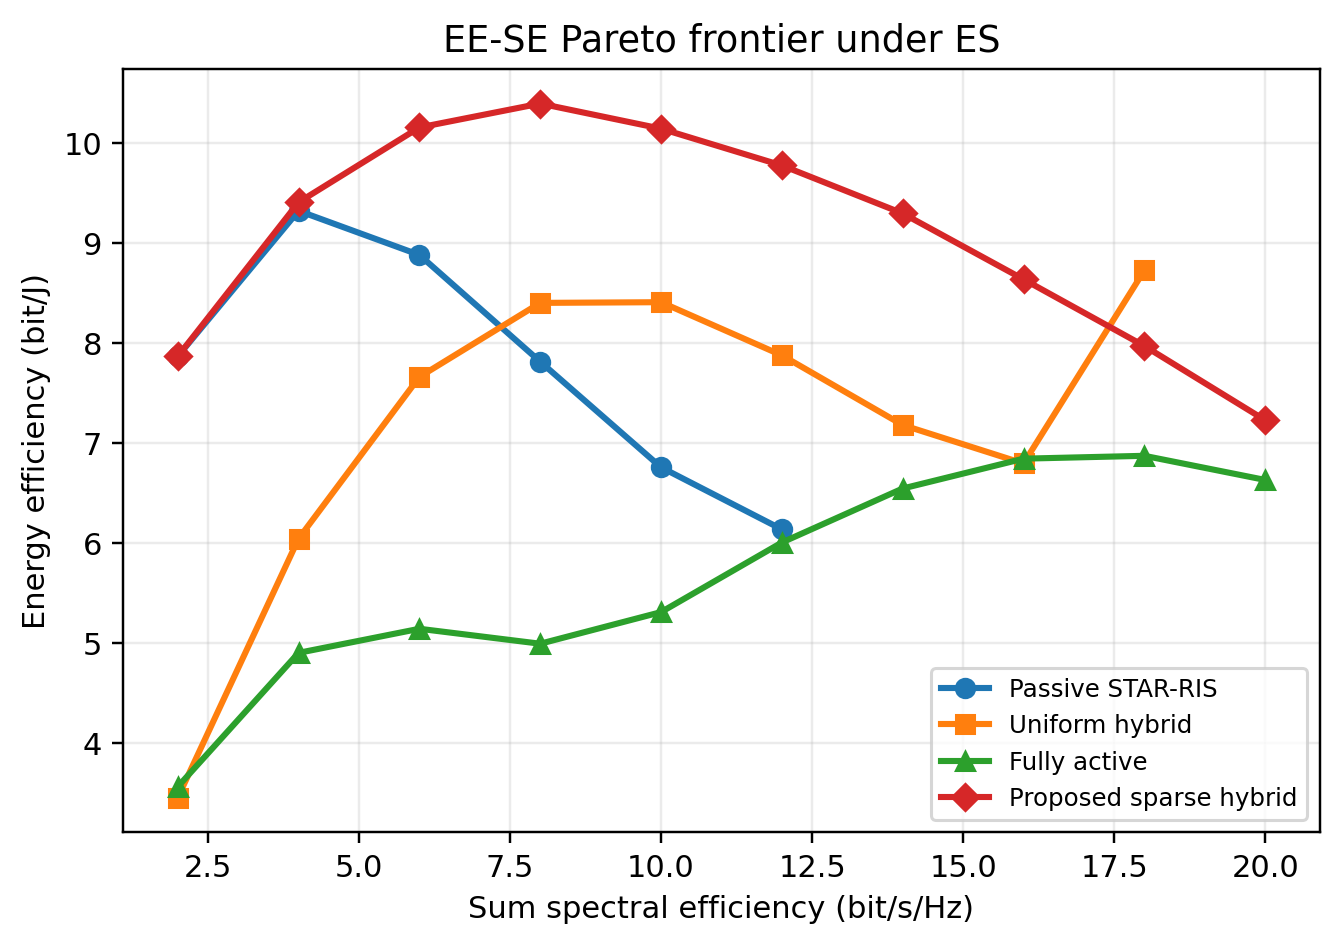
\includegraphics[width=\columnwidth]{fig_pareto_frontier.png}
\caption{Average EE-SE Pareto frontier under ES. Sparse activation dominates the medium/high-SE region, while the passive design is only competitive at low SE.}
\label{fig:pareto}
\end{figure}

Fig. \ref{fig:design} compares the protocol-dependent design rules of the proposed sparse-hybrid solver. TS requires the densest active set because the effective slot targets are inflated by $1/\tau_s$; at $12$ bit/s/Hz its active ratio is about $0.66$, versus about $0.30$ for ES and $0.32$ for SS. ES stays between the two extremes, whereas SS tracks ES at medium and high SE while avoiding the severe TS slot penalty. The gain curves follow the same regime split: TS reaches the gain cap earlier, while ES and SS approach saturation more gradually and become nearly coincident once the high-SE regime dominates.

\begin{figure*}[t]
\centering
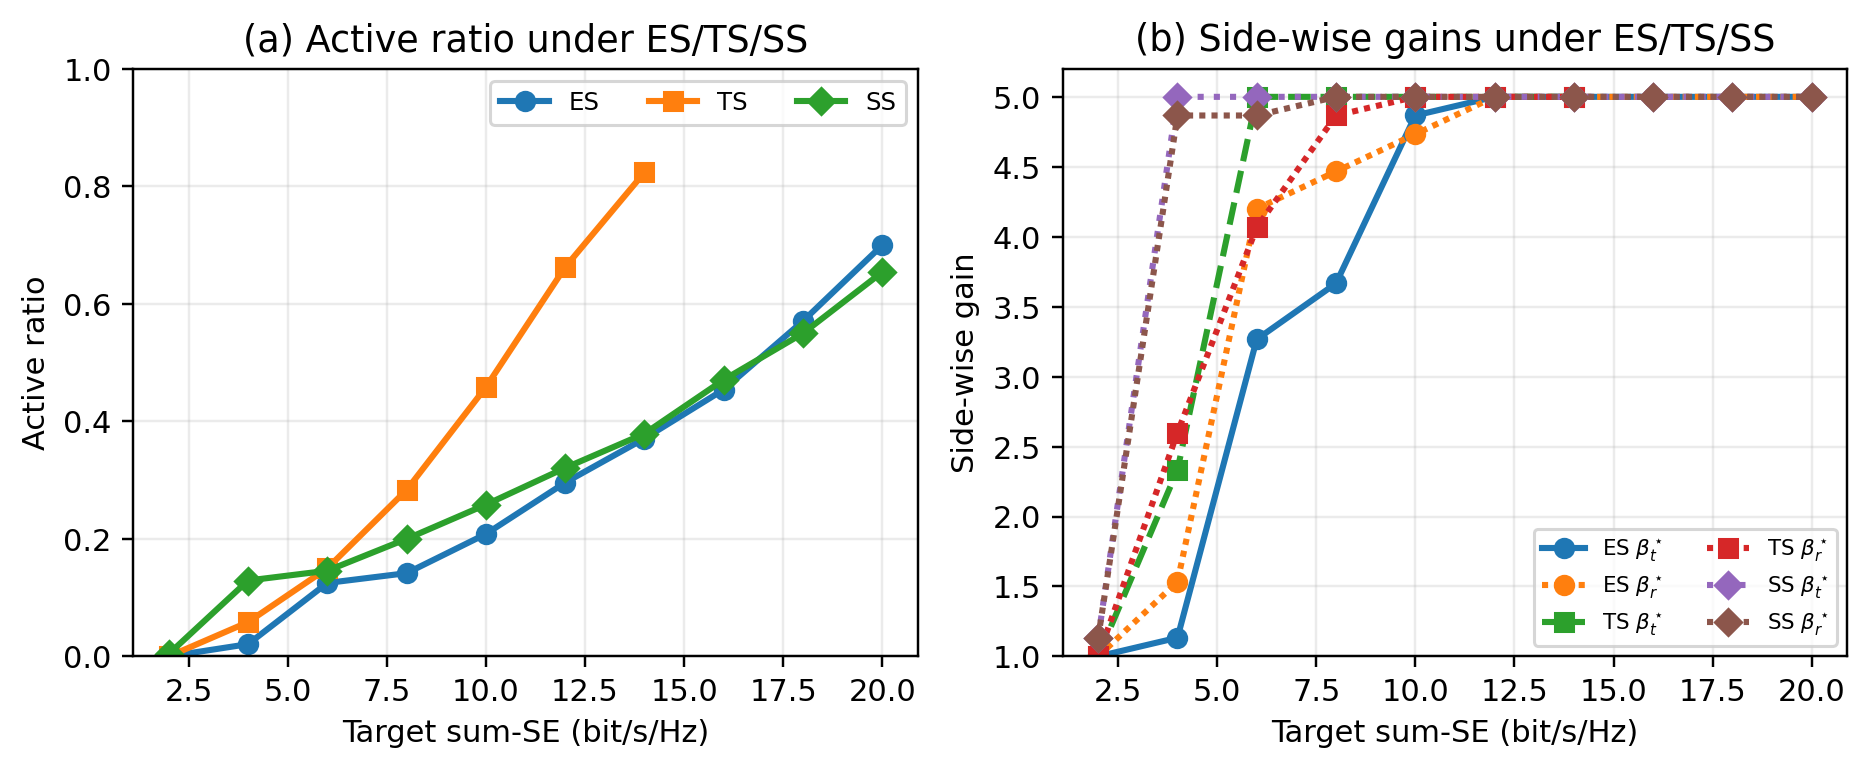
\includegraphics[width=0.92\textwidth]{fig_design_rules.png}
\caption{Protocol-dependent design rules of the proposed sparse-hybrid solver: (a) active ratio versus target SE under ES/TS/SS; (b) side-wise common gains under ES/TS/SS.}
\label{fig:design}
\end{figure*}

Fig. \ref{fig:breakdown} compares the power decomposition at the representative target $R_\Sigma=12$ bit/s/Hz under ES. The fully active design indeed minimizes the BS transmit-power share, but it pays an excessive amplification cost. The passive design has no amplification cost but suffers from a large BS-power term due to the double fading. The proposed sparse-hybrid scheme strikes a better balance: it spends more than passive on hardware, but far less than the fully active design, while sharply reducing the BS radiated-power requirement. This decomposition clarifies why uniform or all-active operation is not EE-optimal.

\begin{figure}[t]
\centering

\includegraphics[width=\columnwidth]{fig_power_breakdown.png}
\caption{Average power breakdown at $R_\Sigma=12$ bit/s/Hz under ES. Sparse activation balances BS transmit and amplification power more efficiently than the benchmarks.}
\label{fig:breakdown}
\end{figure}

Fig. \ref{fig:noise_dyn} compares the hardware sensitivity across ES, TS, and SS at the representative target $R_\Sigma=12$ bit/s/Hz. In Fig. \ref{fig:noise_dyn}(a), the average side-wise gain decreases monotonically with $\sigma_a$ under ES and SS, whereas TS becomes infeasible once $\sigma_a$ exceeds about $0.14$ because the slot-rate inflation already forces a dense active set. Fig. \ref{fig:noise_dyn}(b) shows that increasing the state-update frequency from $50$ Hz to $550$ Hz reduces EE for all three protocols; SS remains the most robust over the whole range, ES follows closely, and TS stays consistently lower because its denser activation pattern magnifies the dynamic-cost penalty.

\begin{figure*}[t]
\centering

\includegraphics[width=0.92\textwidth]{fig_noise_dynamic.png}
\caption{Hardware sensitivity under ES/TS/SS: (a) average side-wise gain versus amplifier-noise level; (b) EE under switching overhead. TS becomes fragile under strong amplifier noise, while ES and SS remain feasible over the tested range.}
\label{fig:noise_dyn}
\end{figure*}

Two additional remarks are worth emphasizing. First, the transmission/reflection asymmetry mainly enters through $(a_s,b_s,d_s)$ and through the rate split $\alpha$; thus the proposed framework remains compatible with user-specific QoS or worst-user constraints. Second, the same active elements can be reused for single-RF calibration or channel sounding: one can augment the score in \eqref{eq:score} with an estimation utility term and impose $|\mathcal{A}|\ge L_{\mathrm{cal}}$, which provides a direct path toward joint calibration/forwarding hardware.

\section{Conclusion}
This paper presented a structured study of the EE-SE tradeoff in hybrid active-passive STAR-RIS. The key contribution is not merely another numerical solver, but an interpretable frontier description connecting amplifier noise, active-set sparsity, side-wise task asymmetry, and hardware power consumption. The analysis yielded a closed-form SE-optimal gain, an explicit active-on threshold, and a simple sparse-activation rule, while the $\epsilon$-constraint algorithm translated these results into a reproducible Pareto-boundary generator. The numerical results showed that the best operating point is rarely fully passive or fully active: low-SE regimes favor passive STAR-RIS, whereas medium/high-SE regimes favor a sparse active subset with carefully controlled gains. Across STAR protocols, TS is more competitive in the low-SE region, ES remains preferable in the intermediate regime, and SS becomes attractive once high-SE operation makes the TS slot penalty dominant. Future work includes exact robust designs with imperfect CSI, joint calibration/forwarding architectures with a single RF chain, and learning-assisted online control for rapidly time-varying STAR-RIS states.


\begin{thebibliography}{99}

\bibitem{direnzo2020smart}
M.~Di Renzo, A.~Zappone, M.~Debbah, M.-S. Alouini, C.~Yuen, J.~de Rosny, and S.~Tretyakov,
``Smart radio environments empowered by reconfigurable intelligent surfaces: How it works, state of research, and the road ahead,''
\emph{IEEE J. Sel. Areas Commun.}, vol.~38, no.~11, pp.~2450--2525, Nov.~2020.

\bibitem{huang2019ee}
C.~Huang, A.~Zappone, G.~C. Alexandropoulos, M.~Debbah, and C.~Yuen,
``Reconfigurable intelligent surfaces for energy efficiency in wireless communication,''
\emph{IEEE Trans. Wireless Commun.}, vol.~18, no.~8, pp.~4157--4170, Aug.~2019.

\bibitem{wu2019irs}
Q.~Wu and R.~Zhang,
``Intelligent reflecting surface enhanced wireless network: Joint active and passive beamforming design,''
\emph{IEEE Trans. Wireless Commun.}, vol.~18, no.~11, pp.~5394--5409, Nov.~2019.

\bibitem{tang2020mimo}
W.~Tang, M.~Z. Chen, X.~Chen, J.~Y. Dai, Y.~Han, M.~Di Renzo, Y.~Zeng, S.~Jin, Q.~Cheng, and T.~J. Cui,
``MIMO transmission through reconfigurable intelligent surface: System design, analysis, and implementation,''
\emph{IEEE J. Sel. Areas Commun.}, vol.~38, no.~11, pp.~2683--2699, Nov.~2020.

\bibitem{liu2021star}
Y.~Liu, X.~Mu, J.~Xu, D.~Niyato, R.~Schober, Y.~L. Guan, and C.~Yuen,
``STAR: Simultaneous transmission and reflection for 360-degree coverage by intelligent surfaces,''
\emph{IEEE Wireless Commun.}, vol.~28, no.~6, pp.~102--109, Dec.~2021.

\bibitem{mu2022star}
X.~Mu, Y.~Liu, L.~Guo, J.~Lin, and R.~Schober,
``Simultaneously transmitting and reflecting (STAR) RIS aided wireless communications,''
\emph{IEEE Trans. Wireless Commun.}, vol.~21, no.~5, pp.~3083--3098, May~2022.

\bibitem{zuo2021noma}
J.~Zuo, Y.~Liu, Z.~Ding, and L.~Song,
``Simultaneously transmitting and reflecting (STAR) RIS assisted NOMA systems,''
in \emph{Proc. IEEE GLOBECOM}, Madrid, Spain, 2021, pp.~1--6.

\bibitem{ma2023activeee}
Y.~Ma, M.~Li, Y.~Liu, Q.~Wu, and Q.~Liu,
``Active reconfigurable intelligent surface for energy efficiency in MU-MISO systems,''
\emph{IEEE Trans. Veh. Technol.}, vol.~72, no.~3, pp.~4103--4107, Mar.~2023.

\bibitem{gao2023active}
Y.~Gao, Q.~Wu, G.~Zhang, W.~Chen, D.~W.~K. Ng, and M.~Di Renzo,
``Beamforming optimization for active intelligent reflecting surface-aided SWIPT,''
\emph{IEEE Trans. Wireless Commun.}, vol.~22, no.~1, pp.~362--378, Jan.~2023.

\bibitem{kunzan2022sub}
K.~Liu, Z.~Zhang, L.~Dai, S.~Xu, and F.~Yang,
``Active reconfigurable intelligent surface: Fully-connected or sub-connected?''
\emph{IEEE Commun. Lett.}, vol.~26, no.~1, pp.~167--171, Jan.~2022.

\bibitem{qi2022sub}
Q.~Zhu, M.~Li, R.~Liu, Y.~Liu, and Q.~Liu,
``Joint beamforming designs for active reconfigurable intelligent surface: A sub-connected array architecture,''
\emph{IEEE Trans. Commun.}, vol.~70, no.~11, pp.~7628--7643, Nov.~2022.

\bibitem{peng2023hybrid}
Q.~Peng, G.~Chen, Q.~Wu, R.~Liu, S.~Ma, and W.~Chen,
``Hybrid active-passive IRS assisted energy-efficient wireless communication,''
\emph{IEEE Commun. Lett.}, vol.~27, no.~8, pp.~2202--2206, Aug.~2023.

\bibitem{huang2024hybrid}
A.~Huang, X.~Mu, L.~Guo, and G.~Zhu,
``Hybrid active-passive RIS transmitter enabled energy-efficient multi-user communications,''
\emph{IEEE Trans. Wireless Commun.}, vol.~23, no.~9, pp.~10653--10666, Sep.~2024.

\bibitem{nguyen2024uav}
N.~T. Nguyen, V.-D. Nguyen, H.~V. Nguyen, Q.~Wu, A.~T"olli, S.~Chatzinotas, and M.~Juntti,
``Fairness enhancement of UAV systems with hybrid active-passive RIS,''
\emph{IEEE Trans. Wireless Commun.}, vol.~23, no.~5, pp.~4379--4396, May~2024.

\bibitem{zhang2022signal}
Z.~Zhang, L.~Dai, X.~Chen, C.~Liu, F.~Yang, R.~Schober, and H.~V. Poor,
``Active RISs: Signal modeling, asymptotic analysis, and beamforming design,''
in \emph{Proc. IEEE GLOBECOM}, Rio de Janeiro, Brazil, 2022, pp.~1--6.

\bibitem{wang2023static}
J.~Wang, W.~Tang, S.~Jin, X.~Li, and M.~Matthaiou,
``Static power consumption modeling and measurement of reconfigurable intelligent surfaces,''
in \emph{Proc. EUSIPCO}, Helsinki, Finland, 2023, pp.~890--894.

\bibitem{wang2024practical}
J.~Wang, W.~Tang, J.~C. Liang, L.~Zhang, J.~Y. Dai, X.~Li, S.~Jin, Q.~Cheng, and T.~J. Cui,
``Reconfigurable intelligent surface: Power consumption modeling and practical measurement validation,''
\emph{IEEE Trans. Commun.}, 2024, doi: 10.1109/TCOMM.2024.3382332.

\bibitem{fotock2024active}
R.~K. Fotock, A.~Zappone, and M.~Di Renzo,
``Energy efficiency optimization in RIS-aided wireless networks: Active versus nearly-passive RIS with global reflection constraints,''
\emph{IEEE Trans. Commun.}, vol.~72, no.~1, pp.~257--272, Jan.~2024.

\bibitem{vu2025hybridstar}
T.-H. Vu, T.~N. Nguyen, T.-T. Nguyen, and S.~Kim,
``Hybrid active-passive STAR-RIS-based NOMA systems: Energy/rate-reliability trade-offs and rate adaptation,''
\emph{IEEE Wireless Commun. Lett.}, vol.~14, no.~1, pp.~238--242, Jan.~2025.

\bibitem{song2025prototype}
R.~Song, H.~Yin, X.~Pei, L.~Cao, T.~Yang, X.~Ren, and Y.-W. Liu,
``Design and prototyping of filtering active STAR-RIS with adjustable power splitting,''
\emph{IEEE Trans. Antennas Propag.}, vol.~73, no.~9, pp.~6462--6476, Sep.~2025.

\bibitem{zhu2025activepassive}
G.~Zhu, X.~Mu, L.~Guo, A.~Huang, and S.~Xu,
``STAR-RIS assisted SWIPT systems: Active or passive?''
\emph{IEEE Trans. Wireless Commun.}, early access, Sep.~2025, doi: 10.1109/TWC.2025.3611793.

\bibitem{soleymani2023starurlcc}
M.~Soleymani, I.~Santamaria, and E.~A. Jorswieck,
``Spectral and energy efficiency maximization of MISO STAR-RIS-assisted URLLC systems,''
\emph{IEEE Access}, vol.~11, pp.~70833--70852, 2023.

\bibitem{xue2023maxmin}
L.~Xue, K.~Wang, Z.~Yang, and M.~Peng,
``Max-min energy-efficiency fair optimization in STAR-RIS assisted communication system,''
\emph{IEEE Access}, vol.~11, pp.~51106--51116, 2023.

\bibitem{zhang2024activestarisac}
S.~Zhang, W.~Hao, G.~Sun, C.~Huang, Z.~Zhu, X.~Li, and C.~Yuen,
``Joint beamforming optimization for active STAR-RIS-assisted ISAC systems,''
\emph{IEEE Trans. Wireless Commun.}, vol.~23, no.~11, pp.~15888--15902, Nov.~2024.

\end{thebibliography}

\end{document}
